\documentclass[a0,portrait]{a0poster}
\usepackage{multicol} % This is so we can have multiple columns of text side-by-side
\columnsep=100pt % This is the amount of white space between the columns in the poster
\columnseprule=3pt % This is the thickness of the black line between the columns in the poster

\usepackage[svgnames,dvipsnames]{xcolor} % Specify colors by their 'svgnames', for a full list of all colors available see here: http://www.latextemplates.com/svgnames-colors
\usepackage{tcolorbox} % coloured boxing of sections
\usepackage{tikz} % manual placement of logos
\usepackage{palatino} % use the Palatino font

\usepackage{graphicx} % Required for including images
\usepackage{enumitem}
\graphicspath{{figures/}} % Location of the graphics files

\usepackage{booktabs} % Top and bottom rules for table
\usepackage[font=small,labelfont=bf]{caption} % Required for specifying captions to tables and figures

\usepackage{amsfonts, amsmath, amsthm, amssymb} % For math fonts, symbols and environments
\usepackage{wrapfig} % Allows wrapping text around tables and figures
\usepackage{mathtools}

\begin{document}
\newcommand{\code}{\texttt}

%----------------------------------------------------------------------------------------
% title and authors
\begin{minipage}[b]{1\linewidth}
	\begin{center}
		\veryHuge \color{DarkRed} \textbf{Using cell colonies for computations} \color{Black}\\ % Title
		\Huge\textit{by reverse-engineering reaction-diffusion systems}\\[2.4cm] % Subtitle
		\huge \textbf{Gregory Sz\'ep, Luca Cardelli, Attila Csik\'asz-Nagy}\\[0.5cm]
		\vspace{1cm}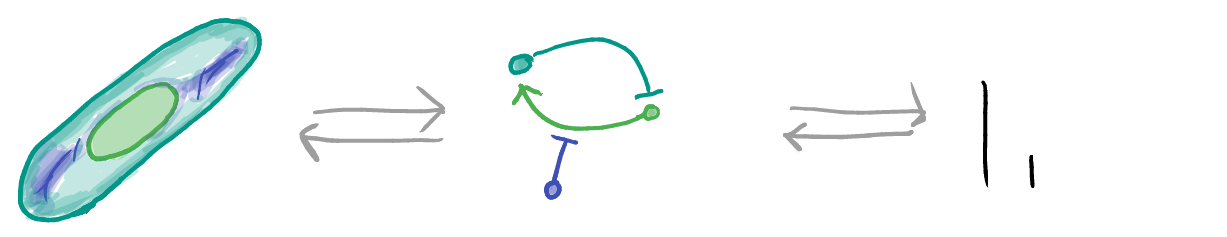
\includegraphics[width=70cm]{abstract}
		\center{mappings between levels of abstraction from biological process to algorithm}
	\end{center}
\end{minipage}

% organisation logos
{\begin{tikzpicture}[remember picture, overlay]
	\node [anchor=north west, inner sep=6cm]  at (-5,36)
		{
\includegraphics[height=7cm]{kcl}};
\end{tikzpicture}}

{\begin{tikzpicture}[remember picture, overlay]
	\node [anchor=north east, inner sep=6cm]  at (79,36)
		{
\includegraphics[height=6cm]{mrc}};
\end{tikzpicture}}

{\begin{tikzpicture}[remember picture, overlay]
	\node [anchor=south west, inner sep=6cm]  at (56,-85)
		{
\includegraphics[height=7cm]{epsrc}};
\end{tikzpicture}}
\LARGE

% figure abstract titles
{\begin{tikzpicture}[remember picture, overlay]
	\node [text width=12cm] at (14,12)
		{\begin{center}\textbf{BIOLOGICAL PROCESS}\end{center}};
\end{tikzpicture}}

{\begin{tikzpicture}[remember picture, overlay]
	\node [text width=12cm] at (40,14)
		{\begin{center}\textbf{DYNAMICAL SYSTEM}\end{center}};
\end{tikzpicture}}

{\begin{tikzpicture}[remember picture, overlay]
	\node [text width=12cm] at (66,17)
		{\begin{center}\textbf{ALGORITHM}\end{center}};
\end{tikzpicture}}

% algorithm code snippet
{\begin{tikzpicture}[remember picture, overlay]
	\node [text width=18cm] at (64.5,23.5)
		{\code{\textbf{
		for \textcolor{DarkBlue}{i} in \textcolor{DarkBlue}{set} : \\
		\qquad do \textcolor{Emerald}{this} ; \\
		\qquad if \textcolor{OliveGreen}{this} then...
		}}};
\end{tikzpicture}}

% arrow captions
{\begin{tikzpicture}[remember picture, overlay]
	\node [text width=12cm] at (24.5,20.5)
		{\begin{center}\textbf{\textcolor{Gray}{synthetic biology}}\end{center}};
\end{tikzpicture}}

{\begin{tikzpicture}[remember picture, overlay]
	\node [text width=10cm] at (23,29)
		{\begin{center}\textbf{\textcolor{Gray}{systems biology}}\end{center}};
\end{tikzpicture}}

{\begin{tikzpicture}[remember picture, overlay]
	\node [text width=10cm] at (47,31)
		{\begin{center}\textbf{\textcolor{Gray}{natural computation}}\end{center}};
\end{tikzpicture}}

\vspace{-16cm}

% itemized thumbs up/down icons
\newcommand*\up{\item[{
\includegraphics[width=0.75em]{up}}\,\,]}
\newcommand*\down{\item[{
\includegraphics[width=0.75em]{down}}\,\,]}

%----------------------------------------------------------------------------------------
 % default text size
Can bacterial colonies perform a fourier transform?
What does a bacteria do? How would we manipulate it?

Bacteria already perform computations
eg chemotaxis, lac system
experimental figure + odes + network

genetic manipulation can supress/activate network segments
We can cut-and-paste different network sections
- synthetic biology approaches

Can we cut-and-paste the right networks together to perform any arbitrary caclulation?

\begin{tcolorbox}[boxrule=2pt,arc=3.4pt,boxsep=2mm]
	\begin{center}
		\textbf{\color{Grey}Algorithm $\rightarrow$ Dynamical System \color{Black}$|$
		Given a \textit{response function} what is the \textit{minimal} reaction network?}
	\end{center}
\end{tcolorbox}

\begin{itemize}[leftmargin=5cm]
	\up Methods for the probabilistic inference of reaction networks exist \cite{Galagali2016BayesianNetworks}
	\up Mappings to and from algorithms pave the path towards programming in cells \cite{Dalchau2018ComputingClocks}
	\down No general mapping exists that takes model complexity into consideration
\end{itemize}

\begin{align*}
	\partial_t\bar{\mathrm{p}}(t)\;\;=
	\overbracket[2pt][10pt]{R(\rho)}^{\text{reaction}}+
	\underbracket[2pt][10pt]{S(t)}_{\text{source}}
\end{align*}
% $R(\rho)$ is a vector, multinomial in the components of $\rho$


%----------------------------------------------------------------------------------------
\begin{multicols}{2}

\begin{tcolorbox}[boxrule=2pt,arc=3.4pt,boxsep=2mm]
	\begin{center}
		\textbf{
		What is the general routine for \textit{reducing complexity} in reaction networks?}
	\end{center}
\end{tcolorbox}

\begin{itemize}[leftmargin=5cm]
	\up For \textit{known time-scale separations} one can reduce models, introducing memory effects~\cite{Phillies2000ProjectionFormalism}
	\down There exist \textit{no relevance determination} methods beyond
	empirical sensitivity analysis~\cite{Cardelli2016NoiseSwitches}
\end{itemize}

\vfill
\columnbreak

\begin{tcolorbox}[boxrule=2pt,arc=3.4pt,boxsep=2mm]
	\begin{center}
		\textbf{
		How does evolution lead to \textit{complexity increase} in network motifs such as switches and clocks?}
	\end{center}
\end{tcolorbox}

\begin{itemize}[leftmargin=5cm]
	\up Relationship between robustness and \\evolvability has been investigated \cite{Daniels2008SloppinessBiology}
	\down Evolutionary relationships between different chemical networks have not been quantified
\end{itemize}

\vfill
\end{multicols}
\vspace{1cm}
%----------------------------------------------------------------------------------------

\begin{tcolorbox}[boxrule=2pt,arc=3.4pt,boxsep=2mm]
	\begin{center}
		\textbf{\color{Grey}Dynamical System \color{Black}$|$
		Given a \textit{steady state pattern} what is the \textit{minimal} reaction-diffusion network?}
	\end{center}
\end{tcolorbox}

\begin{itemize}[leftmargin=5cm]
	\up Dynamics of local equilibria show promising analysis beyond linear stability \cite{Halatek2018}
	\down Need to design attractors in phase space; no description in phase space exists
\end{itemize}

\begin{align*}
	\partial_t\rho(t)\;\;=
	\overbracket[2pt][10pt]{R(\rho)}^{\text{reaction}}+
	\underbracket[2pt][10pt]{D\,\partial_x^2\rho(t)}_{\text{diffusion}}
\end{align*}
$R(\rho)$ is a vector, multinomial in the components of $\rho$

%----------------------------------------------------------------------------------------
\vfill\normalsize

\begin{minipage}[t][][b]{0.99\textwidth}
	\bibliographystyle{style}
	\bibliography{mendeley_v2}
\end{minipage}

\end{document}
